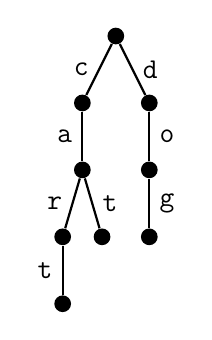
\begin{tikzpicture}[thick,scale=0.5, every node/.style={scale=0.5}, level distance=1.7cm]
    \tikzstyle{marrs}=[very thick,-latex]
    \tikzstyle{tnode}=[circle, fill=black, inner sep=1.5mm]
    \def\rstep{5cm}
    
    \huge
    \tt
    
    \tikzstyle{level 1}=[sibling distance=1.7cm]
    \tikzstyle{level 3}=[sibling distance=1cm]
    
    \node[tnode] {}
        child { node[tnode] {} 
            child { node[tnode] {}
                child { node[tnode] {} 
                    child { node[tnode] {} 
                        edge from parent node[left] {t}
                    }
                    edge from parent node[left] {r}
                }
                child { node[tnode] {} 
                    edge from parent node[right] {t}
                }
                edge from parent node[left] {a}
            }
            edge from parent node[left] {c}
        }
        child { node[tnode] {}
            child { node[tnode] {}
                child { node[tnode] {} 
                    edge from parent node[right] {g}
                }
                edge from parent node[right] {o}
            }
            edge from parent node[right] {d}
        }
        
        ;
    
    
    
    
\end{tikzpicture}